\documentclass[cal1spr16Lectures.tex]{subfiles}

\begin{document}

\section[Week 5]{Week 5: 15-19 Feb}

% % %
\subsection[3.2 Graphing the Derivative]{\S 3.2 Graphing the Derivative}
% % %

% % %
\begin{frame}{\S 3.2 Graphing the Derivative}
Recall: The graph of the derivative is essentially the graph of the collection of slopes of the tangent lines of a graph.  If you just have a graph (without an equation for the graph), the best you can do is approximate the graph of the derivative.
\end{frame}

% % %
\begin{frame}{}{}
%\vspace{1pc}
{\bf Simple Checklist:} 
\begin{itemize}
\item[1. ] Note where $f'(x)=0$.
\item[2. ] Note where $f'(x)>0$. 
\begin{que} What does this look like? \end{que}
\item[3. ] Note where $f'(x)<0$.
\begin{que} What does this look like? \end{que}
\end{itemize}
\end{frame}

% % %
\begin{frame}{}
\begin{ex}
Given the graph of $g(x)$, sketch the graph of $g'(x)$.

\begin{center}
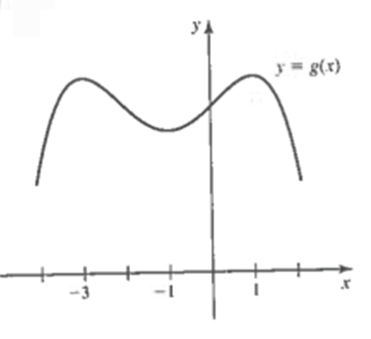
\includegraphics[scale=0.9]{pictures/Ch3Sect2new1}
\end{center}
\end{ex}
\end{frame}

% % %
\begin{frame}
\begin{center}
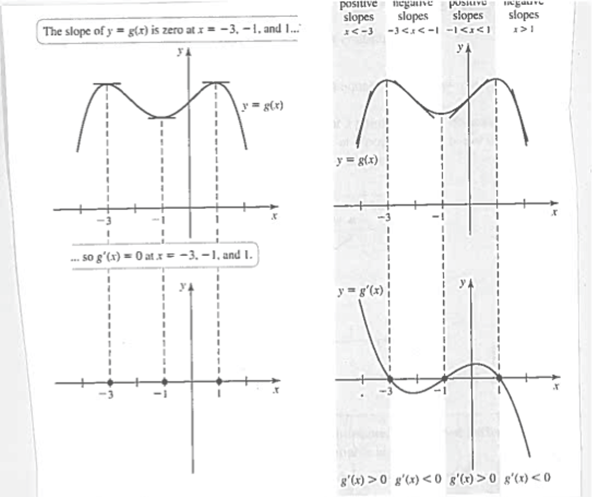
\includegraphics[scale=0.9]{pictures/Ch3Sect2new2}
\end{center}
\end{frame}

% % %
\begin{frame}
\begin{ex}[With Asymptopes]
Given the graph of $f(x)$, sketch the graph of $f'(x)$.

\begin{center}
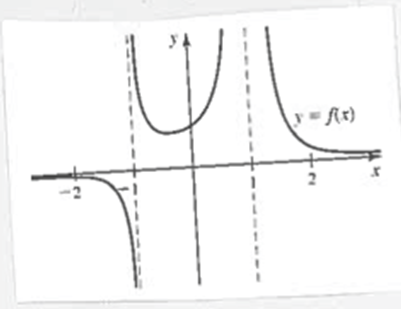
\includegraphics[scale=1]{pictures/Ch3Sect2new3}
\end{center}
\end{ex}
\end{frame}

% % %
\begin{frame}
\begin{center}
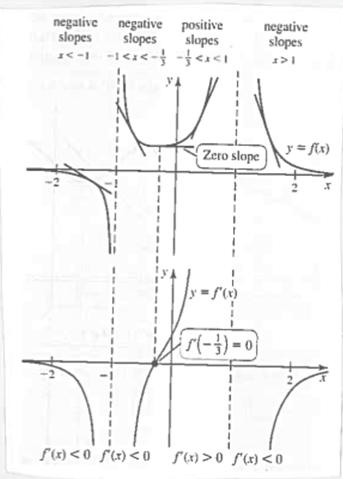
\includegraphics[scale=1]{pictures/Ch3Sect2new4}
\end{center}
\end{frame}

% % %
\begin{frame}
Recall the relationship between differentiability and continuity.
\begin{exe}
If a function $g$ is not continuous at $x=a$, then $g$
\begin{itemize}
\item[A. ] must be undefined at $x=a$.
\item[B. ] is not differentiable at $x=a$.
\item[C. ] has an asymptote at $x=a$.
\item[D. ] all of the above.
\item[E. ] A. and B. only.
\end{itemize}
\end{exe}
\end{frame}

% % %
\subsubsection{Book Problems}
% % %

% % %
\begin{frame}{}
\begin{block}{3.2 Book Problems} 5-14 \end{block} 
\end{frame}

% % % 
\subsection[3.3 Rules of Differentiation]{\S 3.3 Rules of Differentiation}
% % %

% % %
\begin{frame}{\S 3.3 Rules of Differentiation}
Recall the definition of the derivative:
\[f^{\prime}(x)=\lim_{h \to 0} \frac{f(x+h)-f(x)}{h}\]
(as a function of $x$, i.e., a formula).

And, for any particular point $a$, we have 
\[f^{\prime}(a)=\lim_{x \to a} \frac{f(x)-f(a)}{x-a}.\]
\end{frame}

% % %
\subsubsection{Constant Functions}
% % %

% % %
\begin{frame}{\small Constant Functions}\footnotesize
The constant function $f(x)=c$ is a horizontal line with a slope of 0 at every point.  This is consistent with the definition of the derivative:
\begin{align*}
f^{\prime}(x)&=\lim_{h \to 0} \frac{f(x+h)-f(x)}{h} \\
 &=\lim_{h \to 0} \frac{c-c}{h} \\[0.5pc]
 &=\lim_{h \to 0} 0 = 0.
\end{align*}
Therefore, for constant functions, \alert{$\frac{d}{dx}c=0$}.
\end{frame}

% % %
\subsubsection{Power Rule}
% % %

% % %
\begin{frame}{\small Power Rule}{}
{\bf Fact:} For any positive integer $n$, we can factor
\[x^n-a^n=(x-a)(x^{n-1}+x^{n-2}a+\cdots+xa^{n-2}+a^{n-1}).\]

For example, when $n=2$, we get
\[x^2-a^2=(x-a)(x+a),\]
which is the difference of squares formula.
\end{frame}

% % %
\begin{frame}{\small Power Rule, cont.}\footnotesize
Suppose $f(x)=x^n$ where $n$ is a positive integer.  Then at a point $a$,
\begin{align*}
f^{\prime}(a) &= \lim_{x \to a} \frac{f(x)-f(a)}{x-a} = \lim_{x \to a} \frac{x^n - a^n}{x-a} \\[0.25pc]
&= \lim_{x \to a} \frac{(x-a)(x^{n-1}+x^{n-2}a + \dots + xa^{n-2}+a^{n-1})}{x-a} \\[0.25pc]
&= (a^{n-1}+a^{n-2}\cdot a + \dots + a \cdot a^{n-2} + a^{n-1}) = n a^{n-1}. 
\end{align*}
Using the formula for the derivative as a function of $x$, one can show \alert{$\frac{d}{dx} (x^n)= nx^{n-1}$}.
\end{frame}

% % %
\subsubsection{Constant Multiple Rule}
% % %

% % %
\begin{frame}{\small Constant Multiple Rule}
Consider a function of the form $cf(x)$, where $c$ is a constant.  Just like with limits, we can factor out the constant: 
\begin{align*}
\frac{d}{dx}[cf(x)] &= \lim_{h \to 0} \frac{cf(x+h)-cf(x)}{h} \\
&= \lim_{h \to 0} \frac{c[f(x+h)-f(x)]}{h} = c\lim_{h \to 0} \frac{f(x+h)-f(x)}{h} \\[0.25pc]
&= cf^{\prime}(x)
\end{align*}
Therefore, \alert{$\frac{d}{dx}[cf(x)]=cf^{\prime}(x)$}.
\end{frame}

% % %
\subsubsection{Sum Rule}
% % %

% % %
\begin{frame}{\small Sum Rule}
Sums of functions also behave under the same limit laws when we differentiate:
\begin{align*}
\frac{d}{dx}[f(x)+g(x)] &= \lim_{h \to 0} \frac{[f(x+h)+g(x+h)]-[f(x)+g(x)]}{h} \\
&= \lim_{h \to 0} \left[\frac{[f(x+h)-f(x)]}{h}+\frac{[g(x+h)-g(x)]}{h}\right] \\[0.25pc]
&= \lim_{h \to 0} \frac{f(x+h)-f(x)}{h}+ \lim_{h \to 0}\frac{g(x+h)-g(x)}{h} \\[0.25pc]
&= f^{\prime}(x)+g^{\prime}(x)
\end{align*}
\end{frame}

% % %
\begin{frame}{}
So if $f$ and $g$ are differentiable at $x$,
\[\alert{\frac{d}{dx}[f(x)+g(x)]=f^{\prime}(x)+g^{\prime}(x)}.\]
The Sum Rule can be generalized for more than two functions to include $n$ functions.

\vspace{1pc}
{\bf Note:}  Using the Sum Rule and the Constant Multiple Rule produces the Difference Rule:
\[\alert{\frac{d}{dx}[f(x)-g(x)]=f^{\prime}(x)-g^{\prime}(x)}.\]
\end{frame}

% % %
\begin{frame}
\begin{exe}Using the differentiation rules we have discussed, calculate the derivatives of the following functions.  Note which rule(s) you are using.
\begin{itemize}
\item[1.] $y=x^5$
\item[2.] $y=4x^3-2x^2$
\item[3.] $y=-1500$
\item[4.] $y=3x^3-2x+4$
\end{itemize}
\end{exe}
\end{frame}

% % %
\subsubsection{Exponential Functions}
% % %

% % %
\begin{frame}{\small Exponential Functions}\footnotesize
Let $f(x)=b^x$, where $b>0$, $b \neq 1$.  To differentiate at $0$, we write
\[f^{\prime}(0)=\lim_{x \to 0}\frac{f(x)-f(0)}{x-0}=\lim_{x \to 0} \frac{b^x-b^0}{x}=
\lim_{x \to 0} \frac{b^x-1}{x}.\]

\vspace{1pc}
It is not obvious what this limit should be.  However, consider the cases $b=2$ and $b=3$.  By constructing a table of values, we can see that 
\[\lim_{x \to 0} \frac{2^x-1}{x} \approx 0.693 \quad \text{and}\quad \lim_{x \to 0} \frac{3^x-1}{x} \approx 1.099.\]
\end{frame}

% % %
\begin{frame}\footnotesize
So, $f^{\prime}(0)<1$ when $b=2$ and $f^{\prime}(0)>1$ when $b=3$.  As it turns out, there is a particular number $b$, with $2<b<3$, whose graph has a tangent line with slope 1 at $x=0$.  In other words, such a number $b$ has the property that 
\[\lim_{x \to 0} \frac{b^x-1}{x}=1.\]
\begin{que}What number is it? \end{que}
{\bf Answer:} This number is $e=2.718281828459 \dots$ (known as the Euler number).  The function $f(x)=e^x$ is called the \alert{\bf natural exponential function}.
\end{frame}

% % % 
\begin{frame}\footnotesize
Now, using  $\displaystyle\lim_{x \to 0} \frac{e^x-1}{x}=1$, we can find the formula for $\frac{d}{dx}(e^x)$:
\begin{align*}
\alert{\frac{d}{dx}(e^x)} &= \lim_{h \to 0} \frac{e^{x+h}-e^x}{h} \\[0.25pc]
 &= \lim_{h \to 0}\frac{e^x \cdot e^h -e^x}{h} \\[0.25pc]
 &= \lim_{h\to 0}\frac{e^x(e^h-1)}{h} \\[0.25pc]
 &=e^x \left(\lim_{h \to 0} \frac{e^h-1}{h}\right) \\[0.25pc]
  &= e^x \cdot 1 = \alert{e^x}
\end{align*}
\end{frame}

% % %
\begin{frame}{}
\begin{exe} 
	\begin{itemize}
	\item[(a)] Find the slope of the line tangent to the curve $f(x)=x^3-4x-4$ at the point $(2,-4)$. 
	\item[(b)] Where does this curve have a horizontal tangent?
	\end{itemize}
\end{exe}	
\end{frame}

% % %
\subsubsection{Higher-Order Derivatives}
% % %

% % %
\begin{frame}{\small Higher-Order Derivatives}
If we can write the derivative of $f$ as a function of $x$, then we can take \emph{its} derivative, too.  The derivative of the derivative is called the {\bf second derivative} of $f$, and is denoted $f^{\prime\prime}$.  

\vspace{1pc}
In general, we can differentiate $f$ as often as needed.  If we do it $n$ times, the $n$th derivative of $f$ is 
\[\alert{f^{(n)}}(x)=\frac{\alert{d^n} f}{\alert{dx^n}}=\alert{\frac{d}{dx}}[\alert{f^{(n-1)}}(x)].\]
\end{frame}

% % %
\subsubsection{Book Problems}
% % %

% % %
\begin{frame}{}
\begin{block}{3.3 Book Problems} 9-48 (every 3rd problem), 51-53, 58-60 \end{block} 
\begin{itemize}
\item For these problems, use only the rules we have derived so far.
\end{itemize}
\end{frame}

% % %
\subsection[3.4 The Product and Quotient Rules]{\S 3.3 The Product and Quotient Rules}
% % %

% % %
\begin{frame}{\S 3.4 The Product and Quotient Rules}
Issue: Derivatives of products and quotients do \alert{NOT} behave like they do for limits.  
\end{frame}

% % %
\begin{frame}\footnotesize
As an example, consider $f(x)=x^2$ and $g(x)=x^3$.  We can try to differentiate their product in two ways:
\begin{itemize}\footnotesize
\item $\begin{aligned}[t]
	\frac{d}{dx}[f(x)g(x)] &= \frac{d}{dx}\left(x^5 \right) \\[0.25pc]
	 &= 5x^4
	\end{aligned}$
\item $\begin{aligned}[t]
	f^{\prime}(x)g^{\prime}(x) &= (2x)(3x^2) \\
	 &= 6x^3
	 \end{aligned}$
\end{itemize}
\begin{que}Which answer is the correct one? \end{que}
\end{frame}

% % %
\subsubsection{Product Rule}
% % %

% % %
\begin{frame}{\small Product Rule}\footnotesize
If $f$ and $g$ are any two functions that are differentiable at $x$, then
\[\alert{\frac{d}{dx}[f(x) g(x)] = f^{\prime}(x) g(x) + g^{\prime}(x) f(x)}.\]
In the example from the previous slide, we have
\begin{align*}
\frac{d}{dx}[x^2\cdot x^3] &= \frac{d}{dx}(x^2)\cdot (x^3)+x^2\cdot\frac{d}{dx}(x^3) \\
 &= (2x)\cdot (x^3)+x^2\cdot (3x^2) \\[0.25pc]
 &= 2x^4+3x^4 \\[0.25pc]
 &= 5x^4
\end{align*}
\end{frame}

% % %
\subsubsection{Derivation of the Product Rule}
% % %

% % %
\begin{frame}[allowframebreaks]{\small Derivation of the Product Rule}\footnotesize
\begin{align*}
&\frac{d}{dx}[f(x)g(x)] = \lim_{h \to 0} \frac{f(x+h)g(x+h)-f(x)g(x)}{h} \\[1pc]
 =\lim_{h \to 0} &\left(\frac{f(x+h)g(x+h)+\alert{[-f(x)g(x+h)+f(x)g(x+h)]}-f(x)g(x)}{h}\right) \\[0.5pc] 
 =\lim_{h \to 0} &\left(\frac{f(x+h)g(x+h)\alert{-f(x)g(x+h)}}{h}\right) \\
&\hspace{5pc} + \left(\lim_{h \to 0}\frac{\alert{f(x)g(x+h)}-f(x)g(x)}{h}\right) \\[0.5pc]
\end{align*} 

\framebreak
\begin{align*} 
 =\lim_{h \to 0} &\left(g(x+h) \frac{f(x+h)-f(x)}{h}\right) + \left(\lim_{h \to 0} f(x) \frac{g(x+h)-g(x)}{h}\right) \\[0.5pc]
 &=g(x)f^{\prime}(x)+f(x)g^{\prime}(x)
\end{align*}
\end{frame}

% % % 
\begin{frame}
\begin{exe} 
Use the product rule to find the derivative of the function $(x^2+3x)(2x-1)$.
\begin{itemize}
\item[A. ] $2(2x+3)$
\item[B. ] $6x^2+10x-3$
\item[C. ] $2x^3+5x^2-3x$
\item[D. ] $2x(x+3)+x(2x-1)$
\end{itemize}
\end{exe}
\end{frame}

% % %
\subsubsection{Derivation of the Quotient Rule}
% % %

% % %
\begin{frame}{\small Derivation of Quotient Rule}\footnotesize
\begin{que} Let $q(x)=\frac{f(x)}{g(x)}$.  What is $\frac{d}{dx}q(x)$? \end{que}
{\bf Answer:} We can write $f(x)=q(x) g(x)$ and then use the Product Rule:
\[f^{\prime}(x) = q^{\prime}(x) g(x) + g^{\prime}(x) q(x)\] 
and now solve for $q^{\prime}(x)$: 
\[q^{\prime}(x)=\frac{f^{\prime}(x)-q(x)g^{\prime}(x)}{g(x)}.\]
\end{frame} 

% % %
\begin{frame}{}\footnotesize
Then, to get rid of $q(x)$, plug in $\frac{f(x)}{g(x)}$:
\begin{align*}
q^{\prime}(x) &= \frac{f^{\prime}(x)-g^{\prime}(x)\alert{\frac{f(x)}{g(x)}}}{g(x)} \\[0.5pc]
 &= \frac{\alert{g(x)} \left( f^{\prime}(x)-g^{\prime}(x)\frac{f(x)}{g(x)} \right)}{\alert{g(x)}\cdot g(x)} \\[1pc]
\alert{\frac{d}{dx}\left(\frac{f(x)}{g(x)}\right)} & \alert{=\frac{f^{\prime}(x) g(x)-g^{\prime}(x)f(x)}{g(x)^2}}
\end{align*}
``LO-D-HI minus HI-D-LO  over LO squared"
\end{frame}

% % %
\subsubsection{Quotient Rule}
% % %

% % % 
\begin{frame}{\small Quotient Rule}
Just as with the product rule, the derivative of a quotient is not a quotient of derivatives, i.e.
\[\frac{d}{dx} \left[ \frac{f(x)}{g(x)}\right] \ne \frac{f^{\prime}(x)}{g^{\prime}(x)}.\]
Here is the correct rule, the Quotient Rule:
\[\frac{d}{dx} \left[ \frac{f(x)}{g(x)}\right] = \frac{f^{\prime}(x) g(x)-g^{\prime}(x) f(x)}{[g(x)]^2}.\]
\end{frame}

% % %
\begin{frame}
\begin{exe} Use the Quotient Rule to find the derivative of 
\[\frac{4x^3+2x-3}{x+1}.\]
\end{exe}
\begin{exe} Find the slope of the tangent line to the curve 
\[f(x)=\frac{2x-3}{x+1}\text{ at the point }(4,1).\] 
\end{exe}
\end{frame}

% % %
\begin{frame}{}
The Quotient Rule also allows us to extend the Power Rule to negative numbers -- if $n$ is any integer, then 
\[\frac{d}{dx}\left[ x^n \right] = nx^{n-1}.\]
\begin{que} How? \end{que}
\end{frame}

% % %
\begin{frame}
\begin{exe} If $f(x)=\frac{x(3-x)}{2x^2}$, find $f^{\prime}(x).$ \end{exe}
\end{frame}

% % %
\subsubsection{Derivative of $e^{kx}$}
% % %

% % %
\begin{frame}{\small Derivative of $e^{kx}$}
For any real number $k$,
\[\frac{d}{dx} \left( e^{kx} \right) = ke^{kx}.\]
\begin{exe}What is the derivative of $x^2 e^{3x}$? \end{exe}
\end{frame}

% % %
\subsubsection{Rates of Change}
% % %

% % %
\begin{frame}{\small Rates of Change}\footnotesize
The derivative provides information about the instantaneous rate of change of the function being differentiated (compare to the limit of the slopes of the secant lines from \S 2.1).

\vspace{1pc}
For example, suppose that the population of a culture can be modeled by the function $p(t)$.  We can find the instantaneous growth rate of the population at any time $t \ge 0$ by computing $p^{\prime}(t)$ as well as the \alert{\bf steady-state population} (also called the {\bf carrying capacity} of the population).  The steady-state population equals 
\[\lim_{t \to \infty} p(t).\]
\end{frame}

% % %
\subsubsection{Book Problems}
% % %

% % %
\begin{frame}{}
\begin{block}{3.4 Book Problems} 9-49 (every 3rd problem), 57, 59, 63, 75-79 (odds) \end{block} 
\end{frame}

\end{document}